%%%%%%%%%%%%%%%%%%%%%%%%%%%%%%%%%%%%%%%%%%%%
%
% 3: Design Methodology
%
%%%%%%%%%%%%%%%%%%%%%%%%%%%%%%%%%%%%%%%%%%%%

The design and optimization of \DSms through hybridized evolutionary strategies is the
primary goal of this work. Specifically, a hybrid orthogonal genetic algorithm is proposed
to optimize the double input, single output IIR filter design which characterizes \DSm
functionality. This algorithm is shown to be robust with only minimal steady-state
misadjustment. Further, this design methodology is shown to outperform established
classical and contemporary design methods.

%%%%%%%%%%%%%%%%%%%%%%%%%%%%%%%%%%%%%%%%%%%%
%%% Design Methodology
\section{Hybrid Orthogonal Evolutionary Strategy (HOES)}
The Hybrid Orthogonal Evolutionary Strategy (HOES) is quite similar to traditional
evolutionary strategies in that the operating principle of evolving the 'most fit'
individual over successive generations remains unchanged. However, in contrast to
traditional evolutionary strategies, the evolutionary process will not be restricted to
pure stochastic transfer of genetic information between progenitors. The process will be
'hybridized' by intelligently sharing genetic information during reproduction such that
the progeny is optimal given the available genotype. Note that this optimality is defined
by context of the fitness function used to evaluate the population. This hybridization of
the evolutionary process is precisely what allows for faster, more accurate, and more
robust filter designs to be evolved.

Figure \ref{fig:HOES_flow_chart} illustrates the flow of the HOES. Each stage of the HOES
will be addressed in the following sections.

\begin{figure}[htbp]
\centering
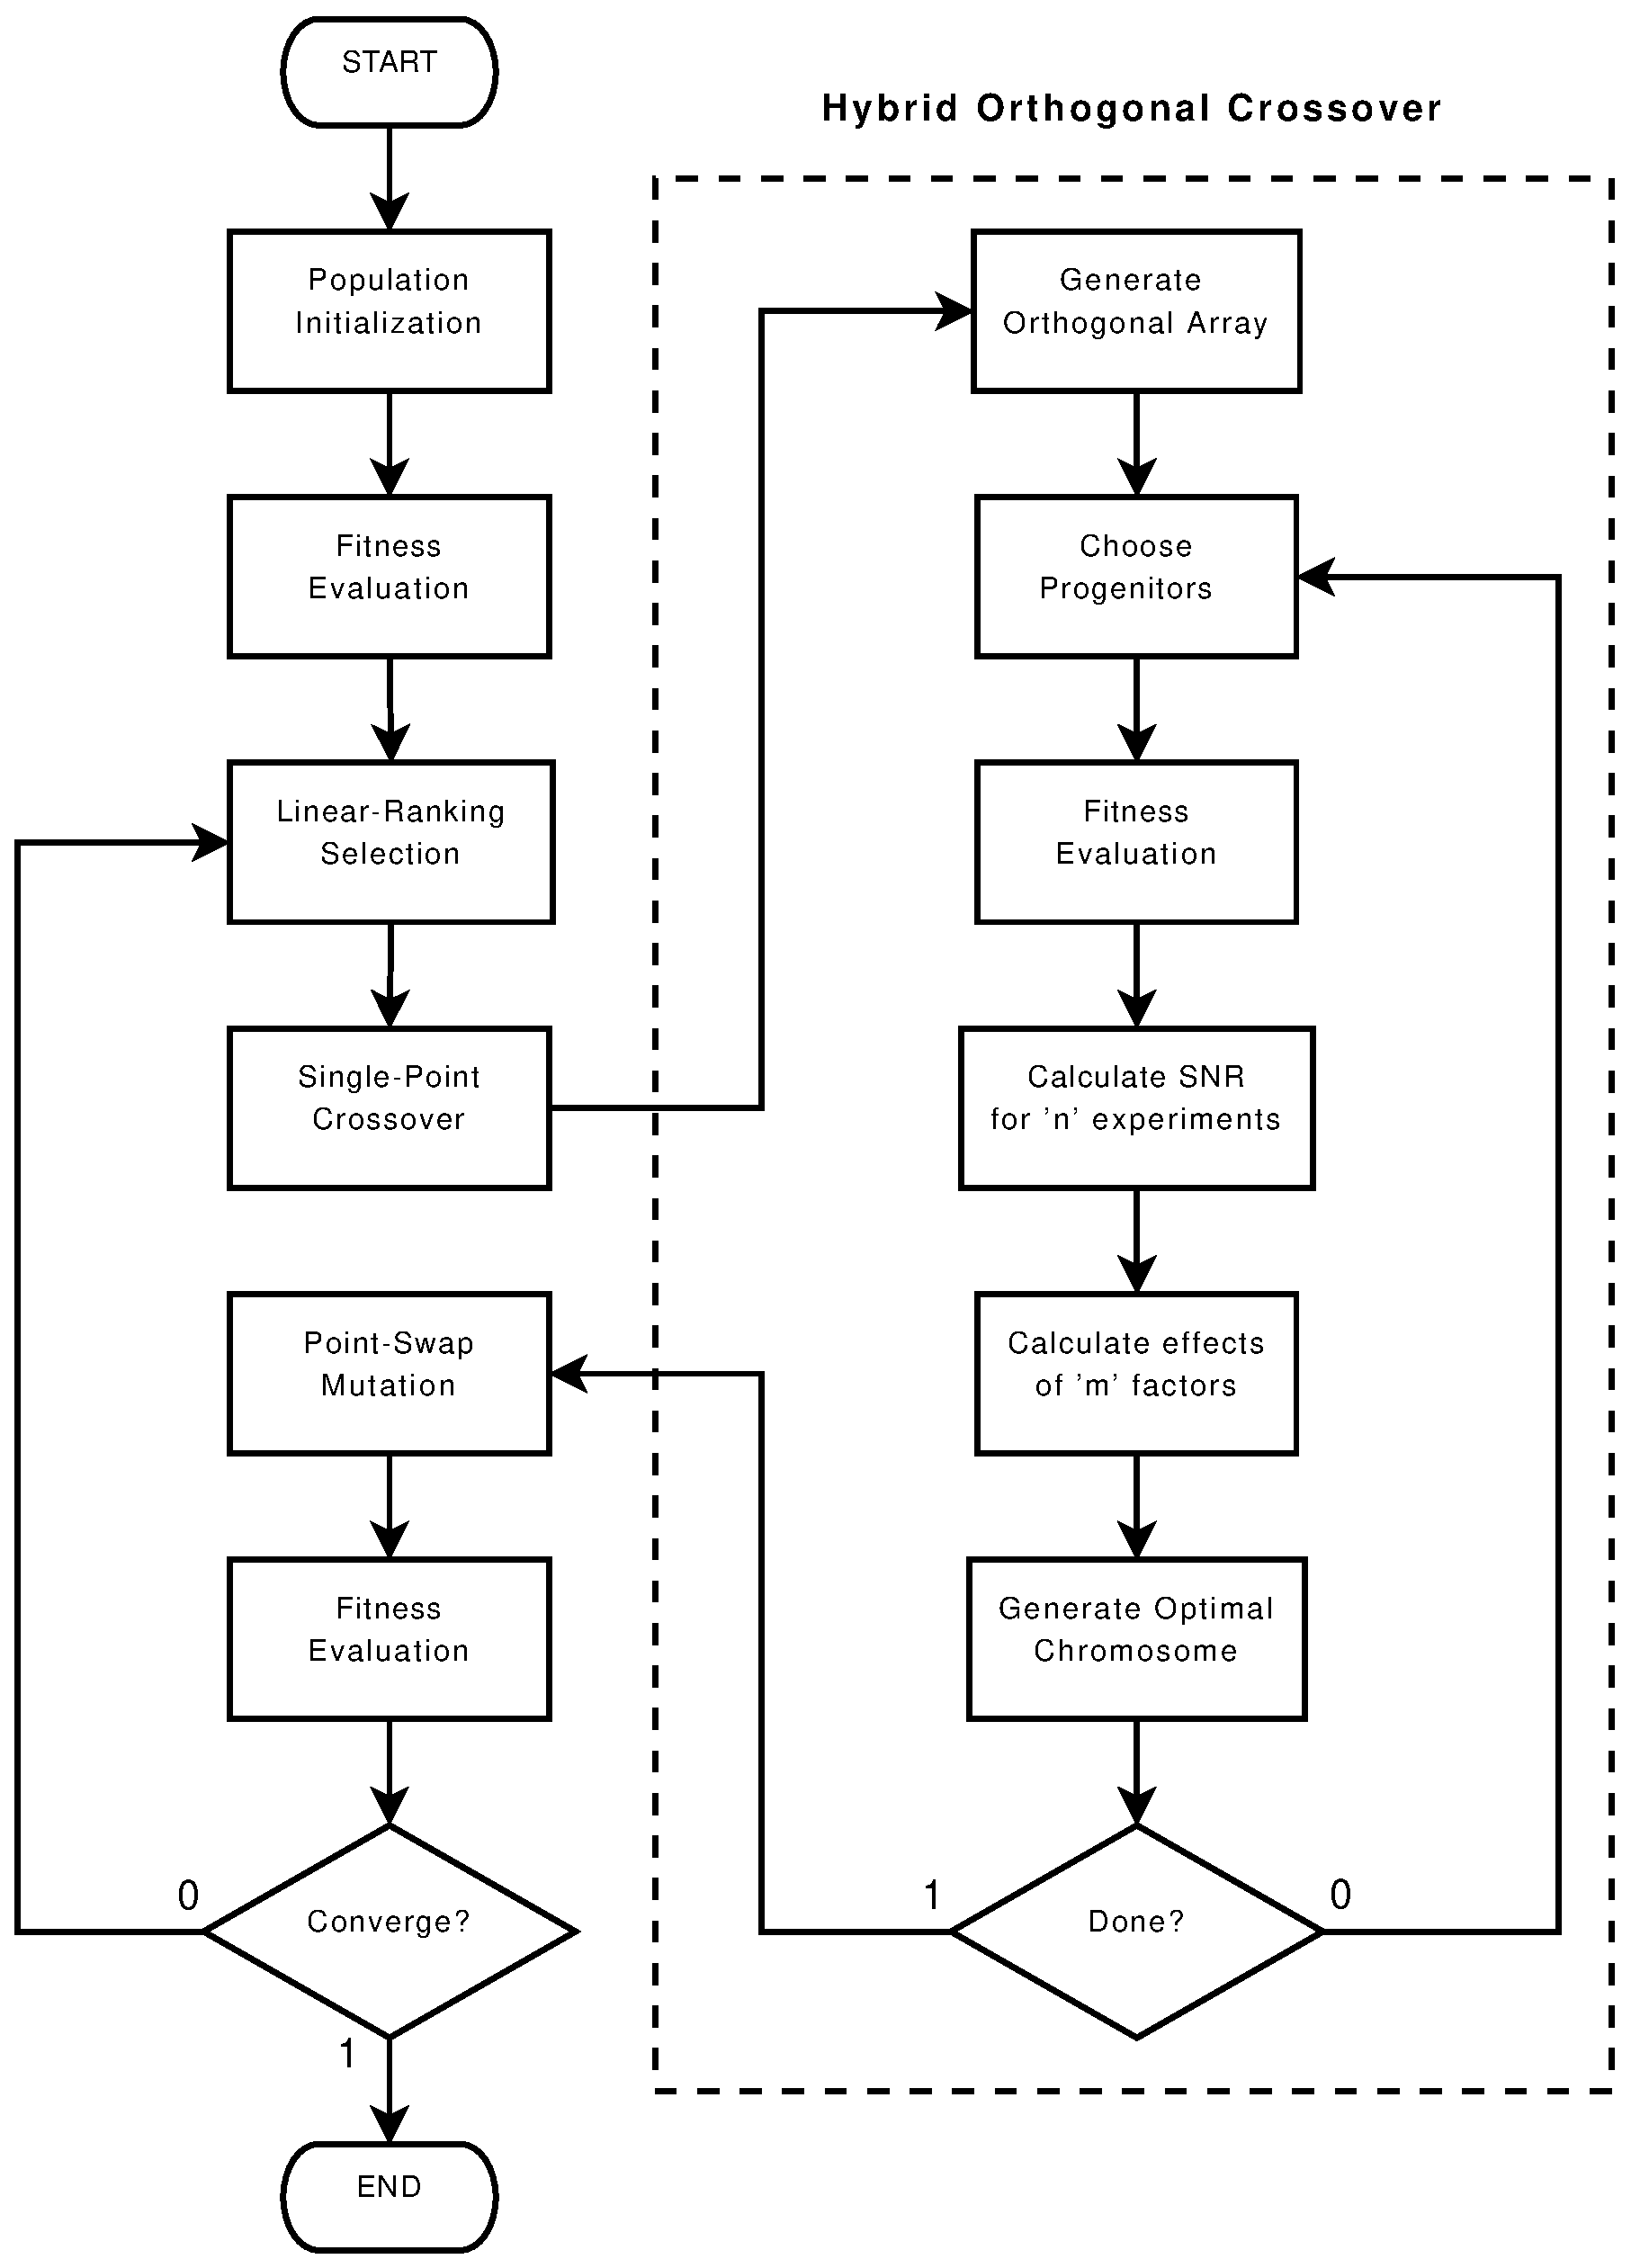
\includegraphics[height=7.5in]{./working_figures/HOES_flow.eps}
\caption{Hybrid Orthogonal Evolutionary Strategy (HOES) Flow Chart}
\label{fig:HOES_flow_chart}
\end{figure}

%%%%%%%%%%%%%%%%%%%%%%%%%%%%%%%%%%%%%%%%%%%%
%%% Chromosome Representation
\subsection{Chromosome Representation}
For every generation, each member of the population is fully characterized by its
chromosome. Specifically, the formulation of this chromosome contains the genetic
information available for reproduction. During reproduction, both traditional and hybrid,
the genetic information contained in the chromosome is exchanged between the progenitors.
This exchange is discussed at length in the following sections.

Structurally, chromosomes are implemented as linear arrays of length $m$. These arrays are
populated with $m$ traits, or alleles, that are iteratively evolved during the
evolutionary process. For this application, the alleles correspond with the coefficients
of the IIR filters which govern the \DSm functionality. Recall that the NTF (and STF) are
designed as IIR filters of the form given in the following equation.
%---------------------
\begin{equation}\label{eq:chromosome_NTF_1}
\textrm{NTF}(z)=\frac{\displaystyle\sum_{i=0}^{M}{a_i
z^{-i}}}{\displaystyle\sum_{i=0}^{M}{b_i z^{-i}}}				
=\frac{\displaystyle\prod_{j=0}^{N}{\bigl(1-c_j z^{-1}\bigr)}}				
		{\displaystyle\prod_{j=0}^{N}{\bigl(1-d_j z^{-1}\bigr)}} 		
\end{equation}
%--------------------- 
Either the polynomial or pole-zero representations shown in \eqref{eq:chromosome_NTF_1}
could be directly implemented in chromosomes where the alleles represent the coefficients.
However, storing the unfactored polynomial coefficients yields chromosomes which are
overly sensitive to perturbation during the evolutionary process. Secondly, implementing
only first order poles and zeros forces the algorithm to directly account for pole-zero
conjugation which significantly lengthens run times. Thus, to reduce coefficient
sensitivity and foster implied conjugation, the chromosomes will be of the following form
\cite{kit-sang_tang_design_1998}.
%---------------------
\begin{equation}\label{eq:chromosome_NTF_2}
\textrm{NTF}(z)=k\displaystyle\prod_{i=0}^{N}\frac{\bigl(1-a_i z^{-1}\bigr)}{\bigl(1-b_i
z^{-1}\bigr)}							
\displaystyle\prod_{j=0}^{M}\frac{\bigl(1+c_{1j}z^{-1}+c_{2j}z^{-2}\bigr)}{\bigl(1+d_{1j}
z^{-1}+d_{2j}z^{-2}\bigr)}	   
\end{equation}
%--------------------- 
Note that one zero-pole pair will exist singularly on the real axis for odd ordered
systems. Thus, $N$ in \eqref{eq:chromosome_NTF_2} is either 1 or 0 for odd or even system
order respectively. Subsequently, the order of the system is then given by the following
equation.
%---------------------
\begin{equation}\label{eq:filter_order}
\text{ORDER}=2M+N	   
\end{equation}
%--------------------- 

The ones are omitted and only the coefficients are stored in the chromosome. As such,
the encoding for even and odd order functions is given by the following expressions where
$\mathcal{C}$ denotes the chromosome.
%---------------------
\begin{subequations}	
\begin{align}
%---------------------
\mathcal{C}_\text{even}&=\bigl[c_{11},c_{12},d_{11},d_{12},c_{21},c_{22},d_{21},d_{22},
\dotsc,c_{M1},c_{M2},d_{M1},d_{M2},k\bigr]\\
\mathcal{C}_\text{odd}&=\bigl[a_1,b_1,c_{11},c_{12},d_{11},d_{12},c_{21},c_{22},d_{21},
d_{22},\dotsc,c_{M1},c_{M2},d_{M1},d_{M2},k\bigr]
%---------------------
\end{align}
\end{subequations}
%---------------------

Note that the length, $m$, of the chromosomes corresponds to the dimension of the
problem space. The system order will be restricted to 8 or less. Thus, the dimension of
the problem space is limited to 33 or less. The proposed algorithm has been tested on
problem dimensions up to 100 and is thus well suited for this application.

%%%%%%%%%%%%%%%%%%%%%%%%%%%%%%%%%%%%%%%%%%%%
%%% Population Initialization
\subsection{Population Initialization}
Recall that global optimization algorithms do not require \textit{a priori} knowledge of
the performance surface shape. However, generalized constraints on the objective function
solution space can greatly increase the speed of algorithm convergence. In fact, seeding
the population with known solutions is often employed as a test for conversion latency. It
has also been shown \cite{sarker_evolutionary_2002} that seeding the population with
solutions which are known to be 'good' or 'approximate' can lead to hyper-accurate
solutions.

Recall that both contemporary and classical designs have zero locations which are 
distributed over the operational region along the unit circle in the complex $z$-domain.
It is therefore assumed that the optimal zero locations will be distributed in some
fashion on or near the unit circle as well. The pole locations, being free to exist
outside of the operational region, will assume a shape geometrically commensurate with the
desired frequency response. Thus, we will assume that the pole and zero locations will be
proximal to both the classical and contemporary results. As such, we will seed the initial
population matrix with dithered chromosomes whose undithered coefficients are given by the
classical Chebyshev polynomial based design approach. The added dither will be a zero mean
standard normal random variable with a fixed variance of 10\% (normalized wrt the unit
circle). The \ith\ dither element is expressed as given in the following equation.
%---------------------
\begin{equation}\label{eq:init_dither}
\delta_{i}=\frac{1}{\sqrt{0.2\pi}}e^{-\frac{x^2}{0.2}}
\end{equation}
%---------------------
Given \eqref{eq:init_dither}, we can express the \ith\ member of the initial population as
a dithered chromosome given as follows.
%---------------------
\begin{equation}\label{eq:dithered_chromosome}
\begin{split}
\mathcal{C}_i&=\bigl[
(c_{11}+\delta_{1}),(c_{12}+\delta_{2}),(d_{11}+\delta_{3}),(d_{12}+\delta_{4}),\dotsc, \\
&\qquad(c_{M1}+\delta_{m-4}),(c_{M2}+\delta_{m-3}),
       (d_{M1}+\delta_{m-2}),(d_{M2}+\delta_{m-1}),(k+\delta_{m}) \bigr]\\
&=\bigl[
\tilde{c}_{11},\tilde{c}_{12},\tilde{d}_{11},\tilde{d}_{12},\tilde{c}_{21},\tilde{c}_{22},
\tilde{d}_{21},\tilde{d}_{22},\dotsc,\tilde{c}_{M1},\tilde{c}_{M2},\tilde{d}_{M1},
\tilde{d}_{M2},\tilde{k}\bigr]
\end{split}
\end{equation}
%---------------------
The initial population is a $m\times n$ matrix whose $n$ columns are the dithered
chromosomes as given in \eqref{eq:init_dither} and $m$ rows correspond to the elements of
the chromosomes. This population matrix, denoted $\mathbb{G}$, is given by the following
equation where $T$ indicates the transpose operation.
\vspace{1mm}
\begin{equation}
\mathbb{G}_{\text{init}} =\bigl[\mathcal{C}_1^T \mathcal{C}_2^T \dotsb
\mathcal{C}_n^T\bigr]=
\begin{pmatrix}
\tilde{a}_{11,1}&\tilde{a}_{11,2}&\hdotsfor{5}&\tilde{a}_{11,n-1}&\tilde{a}_{11,n} \\
\tilde{b}_{12,1}&\tilde{b}_{12,2}&\hdotsfor{5}&\tilde{b}_{12,n-1}&\tilde{b}_{12,n} \\
\tilde{c}_{11,1}&\tilde{c}_{11,2}&\hdotsfor{5}&\tilde{c}_{11,n-1}&\tilde{c}_{11,n} \\
\tilde{c}_{12,1}&\tilde{c}_{12,2}&\hdotsfor{5}&\tilde{c}_{12,n-1}&\tilde{c}_{12,n} \\
\tilde{d}_{11,1}&\tilde{d}_{11,2}&\hdotsfor{5}&\tilde{d}_{11,n-1}&\tilde{d}_{11,n} \\
\tilde{d}_{12,1}&\tilde{d}_{12,2}&\hdotsfor{5}&\tilde{d}_{12,n-1}&\tilde{d}_{12,n} \\
\vdots&\vdots&&&\ddots&&&\vdots&\vdots						   \\
\tilde{c}_{M1,1}&\tilde{c}_{M1,2}&\hdotsfor{5}&\tilde{c}_{M1,n-1}&\tilde{c}_{M1,n} \\
\tilde{c}_{M2,1}&\tilde{c}_{M2,2}&\hdotsfor{5}&\tilde{c}_{M2,n-1}&\tilde{c}_{M2,n} \\
\tilde{d}_{M1,1}&\tilde{d}_{M1,2}&\hdotsfor{5}&\tilde{d}_{M1,n-1}&\tilde{d}_{M1,n} \\
\tilde{d}_{M2,1}&\tilde{d}_{M2,2}&\hdotsfor{5}&\tilde{d}_{M2,n-1}&\tilde{d}_{M2,n} \\
\tilde{k}_{1}&\tilde{k}_{2}&\hdotsfor{5}&\tilde{k}_{n-1}&\tilde{k}_{n} \\
	
\end{pmatrix}
\end{equation}
% \vspace{1mm}

The appropriate sizing for a population is directly related to the complexity of the
problem space. However, this relationship can be difficult, if not impossible, to
adequately characterize \cite{alander_optimal_1992}. Additionally, the relative size of
the population also dictates the nature of the results. For instance, a large
unconstrained population will offer a broad evaluation of the performance surface at the
expense of convergence speed and steady-state misadjustment. In contrast, a smaller
constrained population will converge more quickly at the expense of increased result
diversity.

For generally contrained problem spaces, perhaps the most important concept is minimum
population size. Because minimum population size is tightly coupled with the problem space
complexity, parameters such as this are typically refined or 'tuned' \textit{a posteriori}
\cite{schaffer_-_1989},\cite{alander_optimal_1992}. However, it is also plausible to use
known design parameters applications with similar problem space complexity. Thus, the
initial size of the population has been restricted to 200 for this application and has
proven sufficient for all cases. Note that there are diminishing returns when the
population size becomes prohibitively large. Greatly increasing the population size is
computationally intensive making convergence times unacceptable for most applications.

%%%%%%%%%%%%%%%%%%%%%%%%%%%%%%%%%%%%%%%%%%%%
%%% Fitness Evaluation
\subsection{Fitness Evaluation}
Each member of a population is evaluated for relative fitness during each generation 
(iteration). The result of this fitness evaluation is what drives the evolution of the
greater population. Based on the relative fitness, 'more fit' individuals have an
increased likelyhood of mating and producing offspring thereby preserving their genetic
information in the population genotype. Conversely, 'less fit' individuals have a
decreased likelyhood of mating thereby insuring the elimination of their genetic
information from the population genotype. This process of natural selection according to
relative fitness is central to evolutionary strategies \cite{darwin_origin_2001}.

The algorithm itself is application agnostic and independent of the problem space.
As such, the fitness function (objective function) fully characterizes the problem
space. The objective function discussed here is analogous to the cost function for the
optimization algorithms previously presented. It is the authors opinion that the
evolutionary strategy and the objective function are mutually exclusive. The challenge of
objectifying a particular problem space is wholly independent of the challenge of
architecting an evolutionary strategy.

The various objective functions implemented for the purpose of this work will be
presented in the following sections. However, they are all alike in that they seek to
minimize the result of objective function evaluation (or cost). As such, the HOES evolves
a population whose most fit chromosome represents the global minimum for the respective
objective function. Further, the problem space is generally constrained through the
penalization of chromosomes which evolve outside of the established constraints. The
constraints and respective penalties will also be addressed in the following sections.

%%%%%%%%%%%%%%%%%%%%%%%%%%%%%%%%%%%%%%%%%%%%
%%% Linear-Ranking Selection
\subsection{Linear-Ranking Selection}
As mentioned previously, 'more fit' individuals have a higher likelyhood of reproducing
than 'less fit' individuals. The mechanism which affects this fitness-based
genetic discrimination is referred to as selection. The operating principle for
selection is that a chromosome's probability for mating eligibility is a function of its
fitness with respect to the greater population.

Pure random selection methods suffer from stochastic variability in that there is no
guarantee that all members will be considered for selection. Thus, the possibility exists
that good chromosomes may be inadvertently discarded. Additionally, being application
agnostic, the algorithm assumes that the qualitative 'good vs. bad' indicated by a
particular range of fitness values is sufficient. In practice, however, population
dynamics exist such that the difference between 'good' and 'bad' is poorly reflected in
the observed fitness even for well formed objective functions
\cite{blickle_comparison_1996}.

One method of countering this phenomenon is to implement an 'elitist'
algorithm. By definition, the best chromosome(s) are placed into the next
generation and as well as selected for mating eligibility. This technique has
been shown to greatly increase convergence speeds, especially when steady-state
misadjustment is significant\cite{reeves_genetic_2002}.

Another means of improving selection efficacy is to implement a ranking scheme by
which the population is ordered with respect to its fitness. This ordering removes any
unintended statistical bias from an ill formed objective function. The HOES is a
minimization based evolutionary strategy, and thus the term 'best' corresponds with the
smallest cost. As such, the individuals of a population are sorted according to their
fitness values and the rank 1 is assigned to the worst (highest cost). Similarly, the
rank $N$ is assigned to the best individual (lowest cost) for a population of size $N$.
The probability of selection for mating eligibility is then linearly assigned according
to the individual's rank within the greater population. This is given by the following
equation where $\alpha$ and $\beta$ are positive scalars.
%---------------------
\begin{equation}\label{eq:linear_ranking}
%p_{i}=\frac{1}{N}\left(\eta^{-}+\bigl(\eta^{+}-\eta^{-}\bigr)\frac{i-1}{N-1}\right);
%\quad i\in\{1,\dotsc,N\}
p_{i} = \alpha + \beta i
\end{equation}
%---------------------
Note that $p_{i}$ is a probability and therefore subject to its distribution. Thus,
we can show the following.
%---------------------
\begin{equation}\label{eq:linear_ranking_pdf}
\sum_{i=1}^{N}\bigl(\alpha+\beta i\bigr) = 1
\end{equation}
%---------------------
Solving the summation, we arrive at the following expression.
%---------------------
\begin{equation}\label{eq:linear_ranking_pdf2}
N\left(\alpha + \beta \frac{N+1}{2}\right)=1
\end{equation}
%---------------------

Generally, selection pressure can be defined as the degree of emphasis that is placed on
selecting better suited individuals over worse ones within a given population. As done
here \cite{reeves_genetic_2002}, the selection pressure will be denoted as
$\phi_{x}$ and is described by the following equation.
%---------------------
\begin{equation}\label{eq:linear_ranking_selection}
\phi_{\text{max}} = \frac{p_{\text{max}}}{p_{\text{median}}}
\end{equation}
%---------------------
Substituting \eqref{eq:linear_ranking_pdf2} into \eqref{eq:linear_ranking_selection} we
arrive at the following equation.
%---------------------
\begin{equation}\label{eq:linear_ranking_selection_2}
\phi_{\text{max}} = \frac{\alpha+\beta N}{\alpha+\beta(N+1)/2}
\end{equation}
%---------------------
Finally, solving \eqref{eq:linear_ranking_selection_2} for $\alpha$ and $\beta$ yields
the following expressions.
%---------------------
\begin{subequations}\label{eq:linear_ranking_selection_3}
\begin{align}
\alpha &= \frac{2N-\phi_{\text{max}}\bigl(N+1\bigr)}{N\bigl(N-1\bigr)} \\
\beta  &= \frac{2(\phi_{\text{max}}-1)}{N\bigl(N-1\bigr)}
\end{align}
\end{subequations}
%---------------------
Because $\alpha$ and $\beta$ are positive scalars, it is clear from
\eqref{eq:linear_ranking_selection_3} that $1\leq\phi_{\text{max}}\leq2$. Note that
regardless of individual fitness, the 'most fit' individual is no more than twice as
likely than average to be selected for mating eligibility. A similar analysis can be made
for the relative probability for selection of the 'least fit' individual, denoted as
$\phi_{\text{min}}$.In summary, we can show the following
regarding selection pressure.
%---------------------
\begin{subequations}\label{eq:linear_ranking_phi}
\begin{align}
\phi_{\text{max}} &= 2 - \phi_{\text{min}} \\
\phi_{\text{min}} \geq 0 &\qquad 1\leq\phi_{\text{max}}\leq2
\end{align}
\end{subequations}
%---------------------

In practice, the selection pressure will be fixed such that $\phi_{\text{max}}$
is 1.1\cite{back_optimization_1991}. This provides an adequate balance between exploration
and exploitation of the performance surface. Subsequent to selection, all eligible
chromosomes participate in a stochastic exchange of alleles referred to as crossover.
This will be addressed in the following section.

%%%%%%%%%%%%%%%%%%%%%%%%%%%%%%%%%%%%%%%%%%%%
%%% Single-Point Crossover Operation
\subsection{Single-Point Crossover}
The selection operation generates pool of eligible progenitors as a subset of the current
generation. Randomly selected chromosomes from this 'mating pool' then undergo a
reproductive cycle where alleles are exchanged and offspring are created. This sharing of
genetic information is the vehicle by which fit individuals propagate their beneficial
traits. However, this operation only preserves genetic diversity within the current
generational genotype. There is no new genetic information introduced since only an
exchange of currently available alleles occurs. Thus, if the objective solution does not
exist as some permutation of the currently available genotype, then the crossover
operation will fail to realize the optimal chromosome regardless of the number of
generations.

A great deal of research has been done regarding the mechanism of exchange between two
chromosomes during crossover. Recall that the problem space is fully characterized by the
objective function and that the medium of evaluation is the application specific
chromosome. Prudent design dictates that the structure of the chromosomes is driven
largely by the nature of the objective function. By extension, the optimal process and
manner of allele exchange between chromosomes is an indirect function of problem space
complexity.

For some applications, it may be necessary to carefully regulate which alleles may be
exchanged. These regulations are dictated by the relationships, if any, which exist
between adjacent groups of alleles. However, there is a fine balance between preserving
the stochastic nature of reproduction and the unintended deterministic exchange of
genetic information. The power of evolutionary strategies lies in achieving balance
between exploration of the solution space and exploitation of the localized minima or
maxima. Thus, the structure of the chromosome (which is representative of the problem
space) should be complementary to the crossover method selected.

Single-point crossover has been selected for this application. Single-point
crossover does have positional bias in that it favors continuous segments of genetic
information. However, it does not contain distribution bias as the crossover point is a
discrete random variable with uniform distribution over $\bigl[0,m\bigr]$, where $m$
denotes the length of the respective chromosome\cite{glover_handbook_2003}. Recall that
the alleles represent the coefficients of first and second order polynomials. Thus, there
is no reason to govern the genetic exchange. Further, any exchanges which violate the
underlying algebra will be reflected in the evaluated fitness of the progeny and will be
short lived.

Once the progenitors have been selected, the crossover point is established. All alleles
subsequent to the crossover point are exchanged between the progenitors and two progeny
are created. The single-point crossover process is illustrated in Figure
\ref{fig:crossover} where the progenitor chromosomes are denoted as $\mathcal{C}_x$ and
the progeny chromosomes are denoted as $\mathcal{C}_x^\prime$.
%----------------------------
\begin{figure}[htbp]
\centering
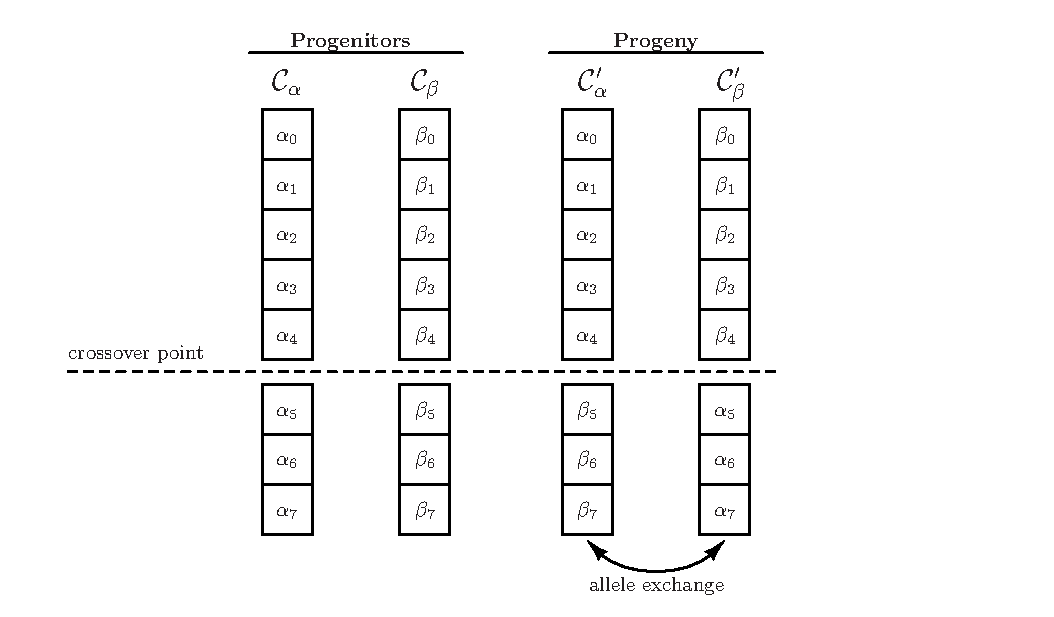
\includegraphics[width=\textwidth]{./final_figures/crossover.eps}
\caption{Single-Point Crossover}
\label{fig:crossover}
\end{figure}
%----------------------------

The process by which individuals are randomly selected is also typically regulated. For
this application, self replication is strictly forbidden. Thus, selected individuals must
crossover with a different individual thereby ensuring the exchange of alleles. This
prevents a single anomalous individual from inadvertently dominating the greater
population which can lead to premature convergence.

%%%%%%%%%%%%%%%%%%%%%%%%%%%%%%%%%%%%%%%%%%%%
%%% Taguchi Method
\subsection{Hybrid Orthogonal Crossover}
The previous sections introduced the traditional operations of selection and crossover.
Typically, the introduction of novel genetic diversity through a mutation operation would
immediatly follow crossover. However, this algorithm will employ an additional hybrid
crossover technique in an effort to intelligently create offspring. Techniques from
biological science and process engineering will be implemented to produce the 'most fit'
individual given the available genotype. Specifically, the Taguchi method of orthogonal
array based design of experiments will be shown to radically improve both solution
accuracy and overall convergence speed.

%%%%%%%%%%%%%%%%%%%%%%%%%%%%%%%%%%%%%%%%%%%%%%%%%%%%%%%%%%%%%%%%%%%%%%%%%%%%%%%%
\subsubsection{Design of Experiments: The Taguchi Method}

%%%%%%%%%%%%%%%%%%%%%%%%%%%%%%%%%%%%%%%%%%%%%%%%%%%%%%%%%%%%%%%%%%%%%%%%%%%%%%%%
\subsubsection{Orthogonal Array Generation}

%%%%%%%%%%%%%%%%%%%%%%%%%%%%%%%%%%%%%%%%%%%%%%%%%%%%%%%%%%%%%%%%%%%%%%%%%%%%%%%%
\subsubsection{SNR Calculations}

%%%%%%%%%%%%%%%%%%%%%%%%%%%%%%%%%%%%%%%%%%%%%%%%%%%%%%%%%%%%%%%%%%%%%%%%%%%%%%%%
\subsubsection{Optimal Progeny Generation}

%%%%%%%%%%%%%%%%%%%%%%%%%%%%%%%%%%%%%%%%%%%%
%%% Point-Swap Mutation
\subsection{Point-Swap Mutation}
'doc stub'

%%%%%%%%%%%%%%%%%%%%%%%%%%%%%%%%%%%%%%%%%%%%
%%% Convergence
\subsection{Convergence}
'doc stub'

%%%%%%%%%%%%%%%%%%%%%%%%%%%%%%%%%%%%%%%%%%%%
%%% DTDSM Design
%%%%%%%%%%%%%%%%%%%%%%%%%%%%%%%%%%%%%%%%%%%%
\section{Discrete-Time \DSM Design}

%%%%%%%%%%%%%%%%%%%%%%%%%%%%%%%%%%%%%%%%%%%%
%%% DTDSM Design: LPNTF
\subsection{Low-Pass NTF Objective Function}'doc stub'
\subsubsection{Initialization}'doc stub'
\subsubsection{Constraints and Penalties}'doc stub'
\subsubsection{Cost Function Characterization}'doc stub'

%%%%%%%%%%%%%%%%%%%%%%%%%%%%%%%%%%%%%%%%%%%%
%%% DTDSM Design: LPSTF
\subsection{Low-Pass STF Objective Function}'doc stub'
\subsubsection{Initialization}'doc stub'
\subsubsection{Constraints and Penalties}'doc stub'
\subsubsection{Cost Function Characterization}'doc stub'

%%%%%%%%%%%%%%%%%%%%%%%%%%%%%%%%%%%%%%%%%%%%
%%% DTDSM Design: VLIF (Bandpass)
\subsection{VLIF Band-Pass Designs}
'doc stub'

%%%%%%%%%%%%%%%%%%%%%%%%%%%%%%%%%%%%%%%%%%%%
%%% DTDSM Design: Output Decimation
\subsection{Output Decimation}
'doc stub'

%%%%%%%%%%%%%%%%%%%%%%%%%%%%%%%%%%%%%%%%%%%%
%%% DTDSM Design: Simulation
\subsection{Simulation}
'doc stub'

%%%%%%%%%%%%%%%%%%%%%%%%%%%%%%%%%%%%%%%%%%%%
%%% CTDSM Design
%%%%%%%%%%%%%%%%%%%%%%%%%%%%%%%%%%%%%%%%%%%%
\section{Continuous-Time \DSM Design}
'doc stub'

%%%%%%%%%%%%%%%%%%%%%%%%%%%%%%%%%%%%%%%%%%%%
%%% CTDSM Design: LPNTF
\subsection{Low-Pass NTF Objective Function}'doc stub'
\subsubsection{Initialization}'doc stub'
\subsubsection{Constraints and Penalties}'doc stub'
\subsubsection{Cost Function Characterization}'doc stub'

%%%%%%%%%%%%%%%%%%%%%%%%%%%%%%%%%%%%%%%%%%%%
%%% CTDSM Design: LPSTF
\subsection{Low-Pass STF Objective Function}'doc stub'
\subsubsection{Initialization}'doc stub'
\subsubsection{Constraints and Penalties}'doc stub'
\subsubsection{Cost Function Characterization}'doc stub'

%%%%%%%%%%%%%%%%%%%%%%%%%%%%%%%%%%%%%%%%%%%%
%%% CTDSM Design: VLIF (Bandpass)
\subsection{VLIF Band-Pass Designs}
'doc stub'

%%%%%%%%%%%%%%%%%%%%%%%%%%%%%%%%%%%%%%%%%%%%
%%% CTDSM Design: Output Decimation
\subsection{Output Decimation}
'doc stub'

%%%%%%%%%%%%%%%%%%%%%%%%%%%%%%%%%%%%%%%%%%%%
%%% CTDSM Design: Simulation
\subsection{Simulation}
'doc stub'